\section{Kommunikationsenhet}
Kommunikationsenheten ansvarar för att förmedla diverse olika sorters information mellan de olika enheterna i systemet. Kommunikationsenheten består av en AVR ATmega16 och en Fireflymodul. Processorn klockas av en 4 MHz klocka som också klockar resten av systemet. 

Kommunikationen mellan PCn och roboten sker via blåtand. Kommunikation mellan de olika delsystemen på roboten sker med en så kallad SPI-buss. SPI-bussens olika anslutningar kan betraktas i figur \ref{fig:spibuss}. Hur de olika pinnarna på processorn är anslutna kan betraktas i figur \ref{fig:PINkomm}.

\begin{figure}[H]
  \centering
 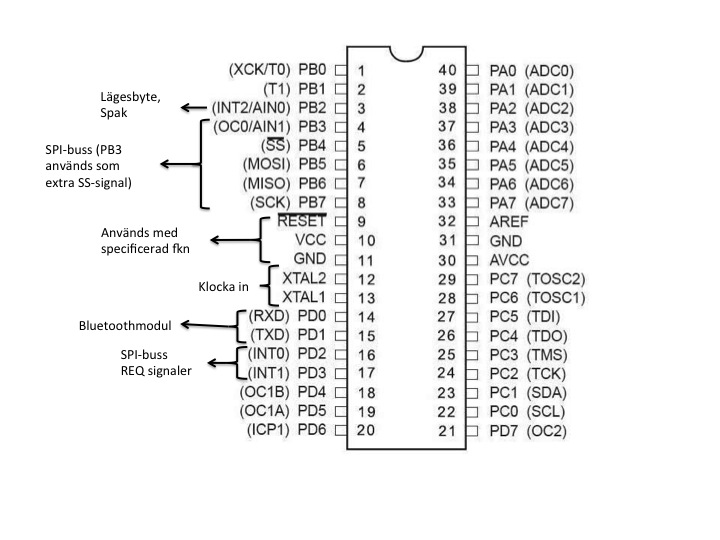
\includegraphics[angle=0,scale=0.5]{bilder/PIN_komm.jpg}
  \caption{Kommunikationsenhetens pin-anslutningar}
  \label{fig:PINkomm}
\end{figure}


\begin{figure}[H]
  \centering
 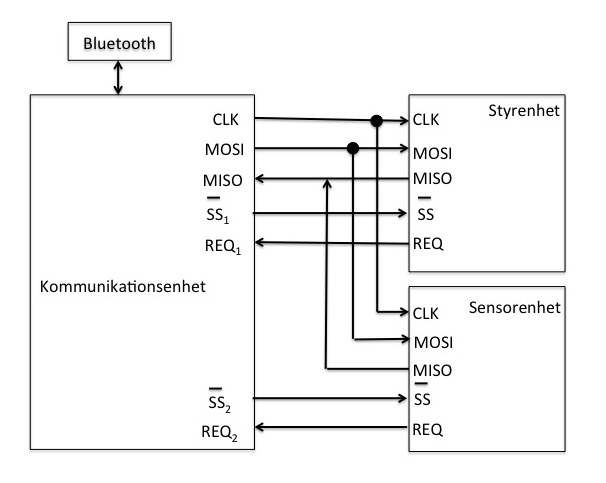
\includegraphics[angle=0,scale=0.5]{bilder/SPI-buss.png}
  \caption{SPI-bussens olika anslutningar}
  \label{fig:spibuss}
\end{figure}


\subsection{Blåtand}
Kommunikationsenheten kommer ha en blåtandsmodul av typ Firefly, ansluten via
UART, för att kommunicera med mjukvaran på PCn.

En blinkande röd LED på blåtandsenheten visar att enheten är redo för en
blåtandsanslutning, medan en stadigt grön LED indikerar att blåtandsenheten har
en aktiv anslutning.

\subsubsection{Överföringar}
Blåtandsenheten kommer att skicka och ta emot information från PCn enligt formatet
8N1, det vill säga att vi skickar data i enheter om 8 bitar (en byte), använder oss
inte av någon paritetsbit samt att vi har en bit som slutbit och en bit som startbit
(som inte anges). Totalt kommer alltså 10 bitar skickas för att överföra 8
bitar. 

Kommunikationsenheten agerar master för SPI-bussen och tar därför emot all data
som skickas mellan systemets olika moduler. För att skicka rätt data till rätt
mottagare så utnyttjar kommunikationsenheten addressfältet i meddelandets
header.

\subsection{SPI}
\label{sec:SPI}
SPI bussen är ett kommunikationssystem som använder ett så kallat Master-Slav system. I robotens system är kommunikationsenheten ensam Master. Systemet har två slavar i form av styrenheten och sensorenheten.
Detta betyder att all kommunikation behöver gå via kommunikationsenheten. SPI-bussen arbetar alltid i så kallat full duplex läge vilket betyder att överföringar kan ske i två riktningar samtidigt. Alla överföringar i systemet sker med två bytes åt gången, en headerbyte som bland annat innehåller adressen och en databyte. För med information om detta, se \ref{sec:Protokoll}. När kommunikationsenheten avslutat en överföring så analyseras alltid headerbyten, som mottagits genom tvåvägskommunikationen, innan nästa externa överföringsefterfrågan behandlas.

Robotens kommunikationssystem fungerar så att styr- och sensorenheten har möjlighet att ta initiativ till överföringar till och från kommunikationsenheten. Detta är inte standard på SPI-bussen utan löses med två stycken extrasignaler, så kallade REQ-signaler. Alla sorters kommunikation kommer att styras med hjälp av avbrott, vilket är ett utmärkt sätt att hantera plötsliga externa kommandon. Då någon av slavarna vill påbörja en överföring sätts enhetens REQ signal hög, vilket genererar ett avbrott hos mastern. Är mastern upptagen då en hög REQ signal skickas så får enheten vänta på att mastern avslutat den pågående överföringen. Efter att mastern blivit uppmärksammad om att en överföring efterfrågas sätts SS-signalen till den berörda enheten låg. Överföringen startas i det ögonblick som mastern skriver något till det temporära SPI-registret, SPDR. I detta ögonblick så börjar mastern också dela ut en klockpuls för överföringen till slavarna. I detta läge och framåt görs ingen skillnad på huruvida det var slaven eller mastern som initierade överföringen. Alla SPI-överföringar avslutas med att en speciell avbrottsflagga, kallad SPIF, sätts. När detta sker kommer båda parterna i överföringen att spara undan den mottagna datan. Då alla SPI överföringar sker med 8 bitar upprepas denna procedur två gånger för varje överföring.

Nedan följer klargöranden om hur de olika portarna i SPI-bussen. 

\subsubsection{SCK}

SCK porten är en port som förmedlar en klocka med en viss frekvens från mastern till de två slavarna. Denna signal bestämmer hur snabbt överföringen ska ske. Klockan kommer börjar skickas då mastern skriver något till dess temporära SPI dataregister, SPDR. När detta skett skickas totalt 8 pulser vilket överför 8 bitar i båda riktningar. Mastern och slaven är konfigurerade för att överföringens olika skeden ska ske samtidigt i klockcykeln. I robotens system används frekvensen 250 kHz, det vill säga 1/16-del av arbetsklockan på 4 MHz för överföringar. Detta är inte den snabbast möjlig överföringshastigheten och kan enkelt förändras vid behov av snabbare överföringar. Den övre begränsningen i överföringshastighet är hälften av arbetsklockan, det vill säga 2 MHz.


\subsubsection{MOSI}
MOSI porten är den port som används när kommunikationsenheten ska skicka 
information till styrenheten och sensorenheten. Den kommer alltså att användas som
input för slavarna och output för mastern. Exempel på information som skickas här är data, med tillhörande header, som skickas till styrenheten från sensorenheten för att reglera de båda hjulens hastighet.

\subsubsection{MISO}
MISO porten används då kommunikationsenheten hämtar information från styr- och sensorenheten. Den är alltså att vara en input för mastern och output för båda slavarna. Exempel på information som skickas med MISO är information om att ett speciellt beslut tagits i sensorenheten. Den header som alltid skickas med specificerar adressen för datat, i detta fall både PCn och styrenheten.
Då all kommunikation med SPI är tvåsidig används även MOSI porten varje gång MISO porten används och viceversa.

\subsubsection{SS}
SS portarna skickar eller tar emot en variant på en chip-select signal. Den SS signal som är låg väljer vilken av slavarna som mastern ska kommunicera med. Endast en av de två SS signalerna får vara låg samtidigt för att undvika busskonflikter. Dessa portar kommer att vara output på kommunikationsenheten och input på styr- och sensorenheten.
En låg SS signal hos någon av slavarna är låg betyder att slavens SPI är aktiverad, förutsatt att nödvändiga bitar satts i slavens SPI-kontrollregister. Överöringens start genererar inget avbrott hos slaven, utan sker istället parallellt med övrig aktivitet hos slaven. Då överföringen avslutats genereras ett avbrott där slaven sparar undan den skickade byten. Är det den första byten i överföringen som skickats får efter det att kommunikationsenheten sparat undan datan och genom en hög REQ signal fått bekräftelse att den berörda slaven gjort detsamma. En enhet som får en hög SS signal kommer att ha sin SPI inaktiv och kommer inte att påverkas av överföringar på bussen.
Efter att två bytes överförts sätts SS signalen åter hög och mastern påbörjar en analys av den skickade headern och om denna specificerar att den mottagna datan ska skickas någonstans.

\subsubsection{REQ}
REQ portarna används av styr- och sensorenheten för att uppmärksamma kommunikationsenheten om att de har ny information att förmedla. När kommunikationsenheten tar emot en signal på någon av REQ portarna kommer det att generera ett avbrott. Under avbrottet kommer SS signalen till enheten som begärt kommunikation att sättas låg och kommunikationen påbörjas. Då mastern kan vara upptagen i det ögonblick då den mottar en hög REQ-signal så låter slavarna REQ-signalen vara hög tills dess att överföringen är färdig då den sätts låg. 

REQ signalen används också för att bekräfta att slavarna sparat undan en headerbyte och är redo att ta emot en databyte.

\subsubsection{Synkronisering}
För att överföringar i systemet ska fungera är det viktigt att masterenhetens och slavenheterernas SPI har samma konfiguration i vissa avseenden. Den kanske viktigaste konfigurationen är vilka moment i överföringen som ska ske på stigande och fallande flank i klockpulsen. I robotens hårdvara finns 4 olika konfigurationslägen. Vilket läge som används kontrolleras av två bitar i ett kontrollregister till respektive enhets SPI. I roboten sätts inte någon av dessa bitar i någon av enheterna.

\subsubsection{Exempel}

När roboten befinner sig i labyrint-läge har sensorenheten gjort en ny avläsning som resulterar i beslutet att en 90\degree kurva är nödvändig. Den vill distribuera denna information vidare. Sensorenheten sätter då en hög utsignal på sin REQ port vilket resulterar i ett avbrott på kommunikationsenheten. Kommunikationsenheten för närvarande är för närvarande upptagen med överföring av reglerdata till styrenheten, så avbrottet får vänta tills denna överföring är klar. Under denna väntan är sensorenhetens REQ signal fortsatt hög.

I avbrottet på kommunikationsenheten så sätts SS signalen till sensorenheten låg, och därefter förmedlar kommunikationsenheten en klockpuls till sensorenheten. När två bytes överförts, en headerbyte och en databyte, så avslutas överföringen och SS signalen till sensorenheten sätts åter hög. Efter att headerbyten tolkats så sätter kommunikationsenheten SS signalen till styrenheten låg, samt genererar en klockpuls till styrenheten. När överföringen av två bytes är färdig sätts SS signalen till styrenheten återigen hög vilket avslutar överföringen. 

Då headerbyten innehöll information om att detta var ett styrbeslut så ska kommunikationsenheten också skicka detta till PCn. Detta görs via en UART port på kommunikationsenheten.

De olika enheternas roll i detta exempel åskådliggörs nedan i ett schema, se figur \ref{fig:schema}.


\begin{figure}[H]
 \centering
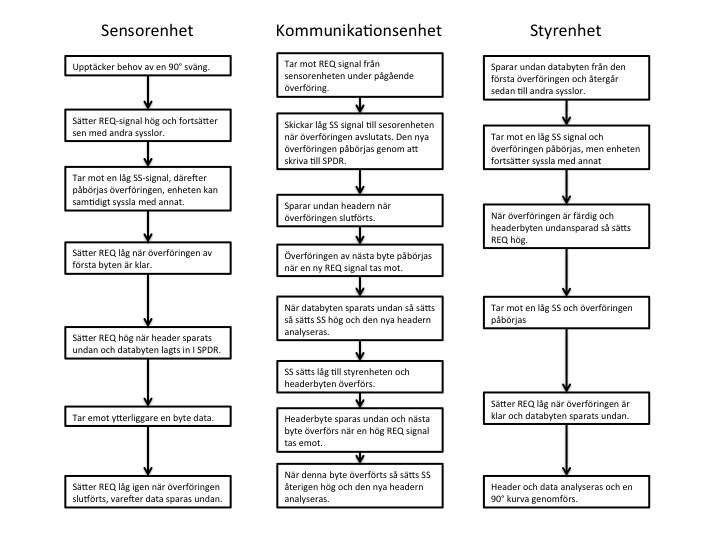
\includegraphics[angle=0,scale=0.7]{bilder/schema_exempel.jpg}
  \caption{Schema över de olika enheternas metodik vid exempelöverföringen}
  \label{fig:schema}
\end{figure}

\subsubsection{Övrigt om kommunikationsenheten}

Som nämnts tidigare kommer det vara kommunikationsenheten som sköter all kontakt mellan PCn och de olika enheterna. Det är på kommunikationsenheten det kommer att finnas en brytare där användaren kan avgöra huruvida denna vill använda roboten i autonomt eller fjärrstyrt läge. Den största skillnaden i kommunikationsenhetens arbete mellan de två lägena är att sensorenheten inte kommer att användas för beslutsfattning i fjärrstyrt läge. Istället kommer alla styrkommandon att skickas till kommunikationsenheten via bluetooth. Kommunikationsenheten kommer också att vara den enhet som tillhandahåller en av- och påknapp för hela systemet.
Vid omställning mellan de olika driftlägena, autonomt och fjärrstyrt, kommer det att överföras ett speciellt kommando till enheterna som beordrar dessa att förändra sina funktioner.  

